% This file was created with tikzplotlib v0.10.1.
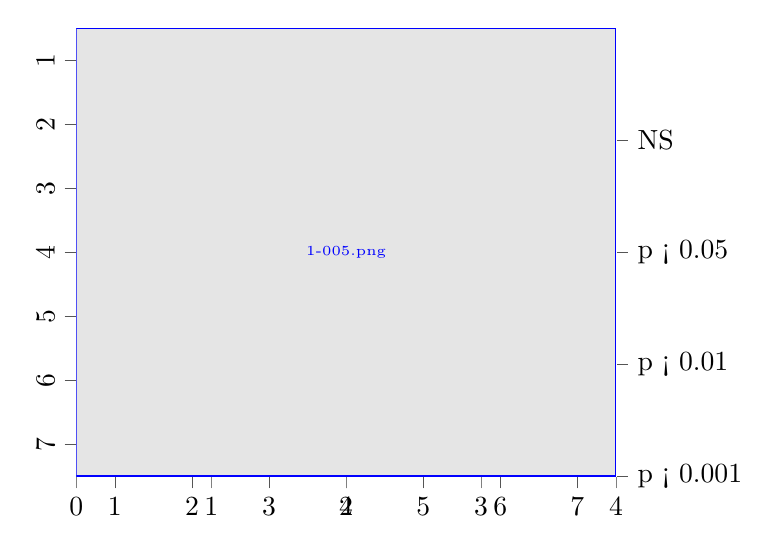
\begin{tikzpicture}

\definecolor{dimgray85}{RGB}{85,85,85}
\definecolor{gainsboro229}{RGB}{229,229,229}

\begin{axis}[
axis background/.style={fill=gainsboro229},
axis line style={white},
tick align=outside,
tick pos=left,
x grid style={white},
xmin=0, xmax=7,
xtick style={color=dimgray85},
xtick={0.5,1.5,2.5,3.5,4.5,5.5,6.5},
xticklabels={1,2,3,4,5,6,7},
y dir=reverse,
y grid style={white},
ymin=0, ymax=7,
ytick style={color=dimgray85},
ytick={0.5,1.5,2.5,3.5,4.5,5.5,6.5},
yticklabel style={rotate=90.0},
yticklabels={1,2,3,4,5,6,7}
]
\addplot graphics [includegraphics cmd=\pgfimage,xmin=0, xmax=7, ymin=7, ymax=0] {1-004.png};
\end{axis}

\begin{axis}[
axis background/.style={fill=gainsboro229},
axis line style={white},
axis y line=right,
tick align=outside,
xmin=0, xmax=4,
xtick pos=left,
y grid style={white},
ymin=0, ymax=4,
ytick pos=right,
ytick style={color=dimgray85},
ytick={0,1,2,3},
yticklabel style={anchor=west},
yticklabels={p < 0.001,p < 0.01,p < 0.05,NS}
]
\path [draw=gainsboro229, fill=gainsboro229, line width=0.004pt]
(axis cs:0,0)
--(axis cs:0,1)
--(axis cs:0,3)
--(axis cs:0,4)
--(axis cs:4,4)
--(axis cs:4,3)
--(axis cs:4,1)
--(axis cs:4,0)
--(axis cs:4,0)
--cycle;
\addplot graphics [includegraphics cmd=\pgfimage,xmin=0, xmax=4, ymin=0, ymax=4] {1-005.png};
\end{axis}

\end{tikzpicture}
